\documentclass[12pt]{article}
\usepackage[margin=0.8in]{geometry}
\usepackage{fancyhdr}
\usepackage{amsmath}
\usepackage{amssymb}
\usepackage{listings}
\usepackage{enumerate}
\usepackage[utf8]{inputenc}
\usepackage{setspace}
\usepackage{graphicx}
\usepackage{hyperref}
\usepackage{float}

\pagestyle{fancy}
\lhead{CS 428}
\chead{Conferenceware Documentation}
\rhead{\today}

%% yay doublespace
\doublespacing
\begin{document}
\renewcommand{\contentsname}{Table of Contents}
\tableofcontents
\newpage

\section{Description}
Conferenceware is a web-based project for running a conference. Specifically, the software was designed to run the ACM Reflections|Projections conference. It is outfitted with features to support everything from registration to event staff scheduling to printing name badges for staff and attendees.  The software was designed to eliminate redundant actions, prevent the introduction of invalid data and, most importantly, make running a large conference easier.

\newpage
%% Nick's WA4
\section{Process}

Our team chose to follow the XP (eXtreme Programming) software development process. The fundamental tenets of this process include pair programming, test first design, user stories, and design simplicity. These tenets give us great flexibility and allow us to make changes to our requirements with minimal refactoring. Additionally changes to requirements can be handled with greater ease in XP because of the emphasis placed on the design of the software. All of these attributes of XP have helped guide our efforts and continue to simplify our workload while allowing individuals or pairs to work concurrently without adverse effects on one another.

From an early stage we have applied pair programming to moderate success. We found that groups of two have helped each other to understand the programming language C\#, which most of us have never used, and the ins and outs of the framework. Our understanding has developed from the ability to bounce ideas off one another to make sense of the intricacies of the framework. In a specific case Brian and I worked together to develop the controller for our speaker object. This controller communicates with our database and has the responsibility of validating data passed to it upon the creation of a speaker in the schema. We also avoided errors in our implementation of the controller because we checked each other's code as we wrote it. Simple formatting or typing errors that a compiler would catch, at the cost of time, did not make it into our code because the constant checks we employed on each other.

Our combined effort also helped us solve issues with third party tools that neither of us had used before. Testing of our work necessitated the use of Microsoft SQL Server. A lightweight version of SQL Server (SQL Server Express) installed with our IDE (Integrated Development Environment). This version of SQL Server did not come with the usual suite of tools that make creating and populating databases easy, so we had to learn how to do this from the command line interface that comes with the product. This put both of our skills to the test as I tend to favor graphical user interfaces in the windows environment and my partner generally works at the command line on UNIX based systems. I had to use my knowledge of typical design patterns employed by Microsoft combined with my partner's familiarity with command line tools.

On a larger scale our choice to work in close proximity has allowed us to debug each other's work and provide help insights that have saved individuals from relearning parts of the framework that someone else already figured out. This constant feedback has sped up development immeasurably and continues to shape our groups coding practice. As the code base continues to grow pair programming and constant group communication will serve as a means of enforcing conformity to our coding standard and insure that the simplicity of the code is maintained.

Our focus on test first design has also helped define the direction of the project. Writing our tests first allows us to think critically about how all the pieces of our design fit together. Writing tests for individual pieces is relatively simple to do, which makes this style of design very appealing. If we find that we need to change the requirements or functionality of the code, whether mandated by knowledge discovered through design of the tests or by our end user, these changes will be simple to make because we have written the tests first and not the actual code. Once we have our tests in place we can begin crafting the code, and we can do periodical checks that our code behaves as desired by running the tests.

Creating the unit tests first also gives us a good feel for our progress as we continue development. Each method that we create that fulfills a unit test brings us one step closer to the completion of the project and everyone can see that progress explicitly. The on the flip side of that coin that means that everyone knows what still needs to be accomplished. We can define goals for individuals or pairs to create the functionality demanded by the tests, and once we know that the goal has been accomplished once we can double check our progress with our tests.

Just because we created our tests at the beginning does not mean that we stop creating tests as the project progresses. We have added tests as we go to insure that we cover as much of the code as possible, and when these situations do arise we take the opportunity to reassess our design. Our ability to reassess our design adds to the flexibility provided to us by XP. Continual checks on our progress have aided our understanding of our requirements as well. All these aspects of testing have made XP an invaluable tool in the construction of our system.

XP has helped guide our development through user stories in addition to the testing already discussed. Our user stories have benefited us greatly particularly because as opposed to many groups we have an actual end user that will be using our product once we have finished working on it. We can communicate with these users regularly to determine if our work fulfills their desire for the final product. It also helps that our end users have had experience and know many of the pitfalls that may arise in the project. Our project will simply generalize much of the work that has been done by the end user over the past few years so that in the future the deployment of the final product need not be a stressful ordeal. Using this goal of eliminating stress on the part of our end user gives our project much needed focus, and the end user experience helps us avoid mistakes they have made in the past.

User stories and the tasks that go with them also help break the project into more manageable chunks. We can distribute these bite size pieces among the group and allow each member to have feature ownership, but still keep a sense of collective ownership of the whole. The tasks allow us to see how individual pieces should come together to fulfill a user story, and that abstraction allows for us to meet our goal of design simplicity. This simplicity becomes evident in that complex dependencies have been minimized, and reusable code snippets become plentiful.

Tying back to the idea of flexibility in requirements, we have tailored our user stories to those requirements that are the most independent. We cannot eliminate all interdependence among our stories, but we can minimize those dependencies. If a user story changes at a late point in development, we should be able to implement those changes with the least amount of work possible. This includes avoiding cascading changes to the code. One requirement change should not force us to change large portions of the code to implement the change. This should also mean that test we wrote before the change should hold after we change the code. Some test will have to change as well, but we can't avoid that. 

The final tenet of XP that plays a significant role in our project is design simplicity. While some of the other tenets already facilitate that goal, design simplicity deserves its own category because of the decision required to keep things simple. One of the most important principles in keeping any design simple requires keeping the length of methods as short as possible. Not only does this give us a better idea of where the code faulted, should we find bugs, but it encapsulates the smallest actions that are performed together routinely. We can then use these over and over without rewriting code that does essentially the same thing over and over. Applying rules for clean code such as short methods and limited nesting increases code readability. This helps us to debug each other's code because we can better read and understand code that someone wrote cleanly without long convoluted functions. 

Design simplicity also applies to the design and structure of the classes and larger hierarchies of the code. Organization of namespaces and classes allows outside viewers of the product to get a better understanding of what pieces do what without needing to look at all of them individually. A passive observer knows that a class designated as a factory will create instances of certain classes without needing to know how those classes are made. He knows that if that class resides within a kernel namespace then that class has something to do with the internal core workings of the program, but he does not need to know more than that. 

This simplicity of the design also allows for easy refactorings of the code. If one has a good understanding of the code, they can more easily make changes to the code that won't break other functionality. These refactortings should also be simple in design and fit together with the rest of the system if the system exhibits high modularity.

In total these four aspects make up the basis of sound software design methodology. XP's relies on these tenets to insure that a team of engineers are working as effectively as possible toward completing the project on time and in a form that is highly maintainable.

\newpage
%% copied in user stories for now
\section{Requirements and Specifications}
\subsection{Public features}
\subsubsection{Register for Roles}
The user will visit the web site and click on the appropriate registration link.
They will then fill in their information and click submit. After submission,
they will be told of the success or failure (due to technical difficulties or
invalid information). Upon success they will also get an email. This should be
possible for attendees, volunteers, and MechMania teams.
\subsubsection{Volunteers can Sign up for Timeslots}
During registration as a volunteer (described above) volunteers need to be able
to choose which time slots they would be willing to work. The registration form
will provide extra information about the role as well as a series of checkboxes
to choose which time slots are available for them to be scheduled.
\subsubsection{Event Listing}
The user will visit the web site and click on events. The events will be
listed in chronological order from top to bottom. Each entry will list the
event title, location, presenter or presenters and time. Clicking the title
will give more details about the event.
\subsubsection{Limited Space Event Registration}
The user will visit the web site and navigate to a specific event. If the event
has limited attendance, this will be expressed. If all available spots are
registered, the user will be informed on the page. If not, a space where an
email address will be provided is listed. The user will enter their email
address. If correct and the user is registered for the conference, success will
be displayed and the user will be emailed. If an error occurs, the user will be
informed and reminded they must register first.

\subsection{Private (administrator) features}
\subsubsection{Insallation}
An Admin will need to be able to install the application. This includes setting up the database
and prefilling certain variables with user defined attributes. This process should involve the least
amount of direct configuration by the user.
\subsubsection{Company Management}
An administrator will have the ability to enter companies into the system manually. From there
an administrator can update the status on the generated invoice. Balances can be marked as
billed or paid, and the system can accept multiple payment sources.
\subsubsection{Billing Companies}
The admin will log into the web site. They will choose to see a list of
companies. They will then choose the appropriate company to bill. They will
add items to the invoice and select which people associated with that company
to send it to. The admin will then submit the invoice which will be emailed
to the people.
\subsubsection{Badge Generation}
The admin is presented with a list of registered attendees, they may select
individually or select all of them. The list is submitted via a web form,
and the server generates and returns a PDF based on the selected users. If
no users were selected, the admin is given an error message. Otherwise, the
web server returns a PDF to the admin, which they can then save, open, or
print.
\subsubsection{Event Creation}
The administrator will login to the Conferenceware website.  They will navigate to an event list.  They will click "Add New Event".  They'll be presented with a clean interface in which to enter any necessary information for an event's creation.  The admin will click "Save" (or "Add", "Create", etc.) and the event will be added to the conference.  The admin will be returned to the list of events.
\subsubsection{Scheduling}
The administrator will login to the Conferenceware website.  They will navigate to the Schedule page.  They will drag an event from the list of events onto the list of available timeslots, choosing where they'd like to place the event in the schedule.  The admin will click on "Save" and the schedule will be saved.
\subsubsection{User Management}
The administrator will log into the Conferenceware website. They will navigate
to the administration section and click on the type of user they would like to
manage. From here, they should be able to create, delete, and edit any user.
\subsubsection{Content Management}
The administrator will log into the Conferenceware website. They will navigate
to the administrative list of events and select to edit a single event. The
administrator will be allowed to upload content or link to content for the
event. Any linked content will now display at the bottom of the event listing.

\subsection{Combination features}
\subsubsection{Form processing}
The user uses a web form to type in their information. The web form is
validated using Javascript and the user is alerted of any necessary
corrections. If correct, the server takes the information, sanitizes it,
and stores it in the database. The server then returns a sucess message
to the user.

%% Oh god, importing pdfs
\section{Architecture and Design}
\subsection{UML Sequence Diagrams}
\begin{figure}[H]
\centering
\caption{Add Event Sequence Diagram}
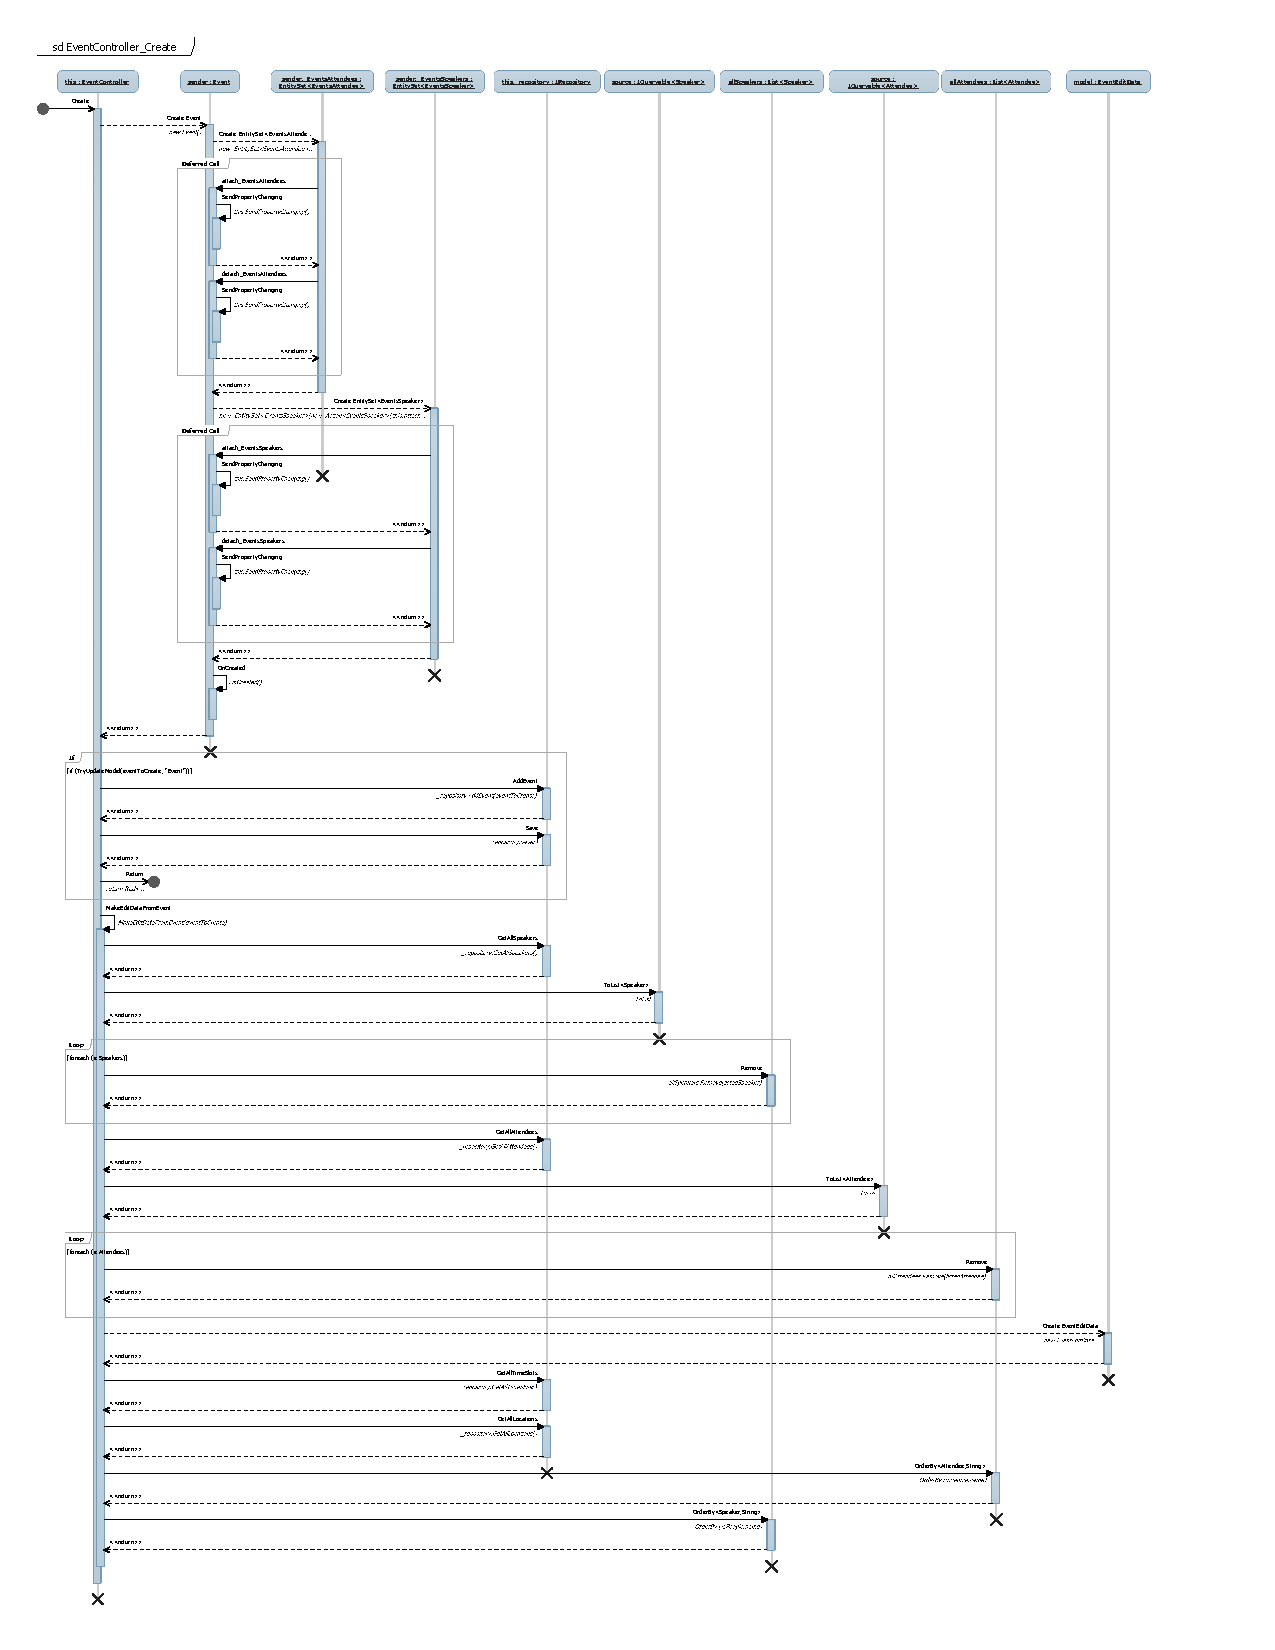
\includegraphics[scale=0.7]{AddEvent_sequence}
\end{figure}
\newpage
\begin{figure}[H]
\centering
\caption{Manage Event Sequence Diagram}
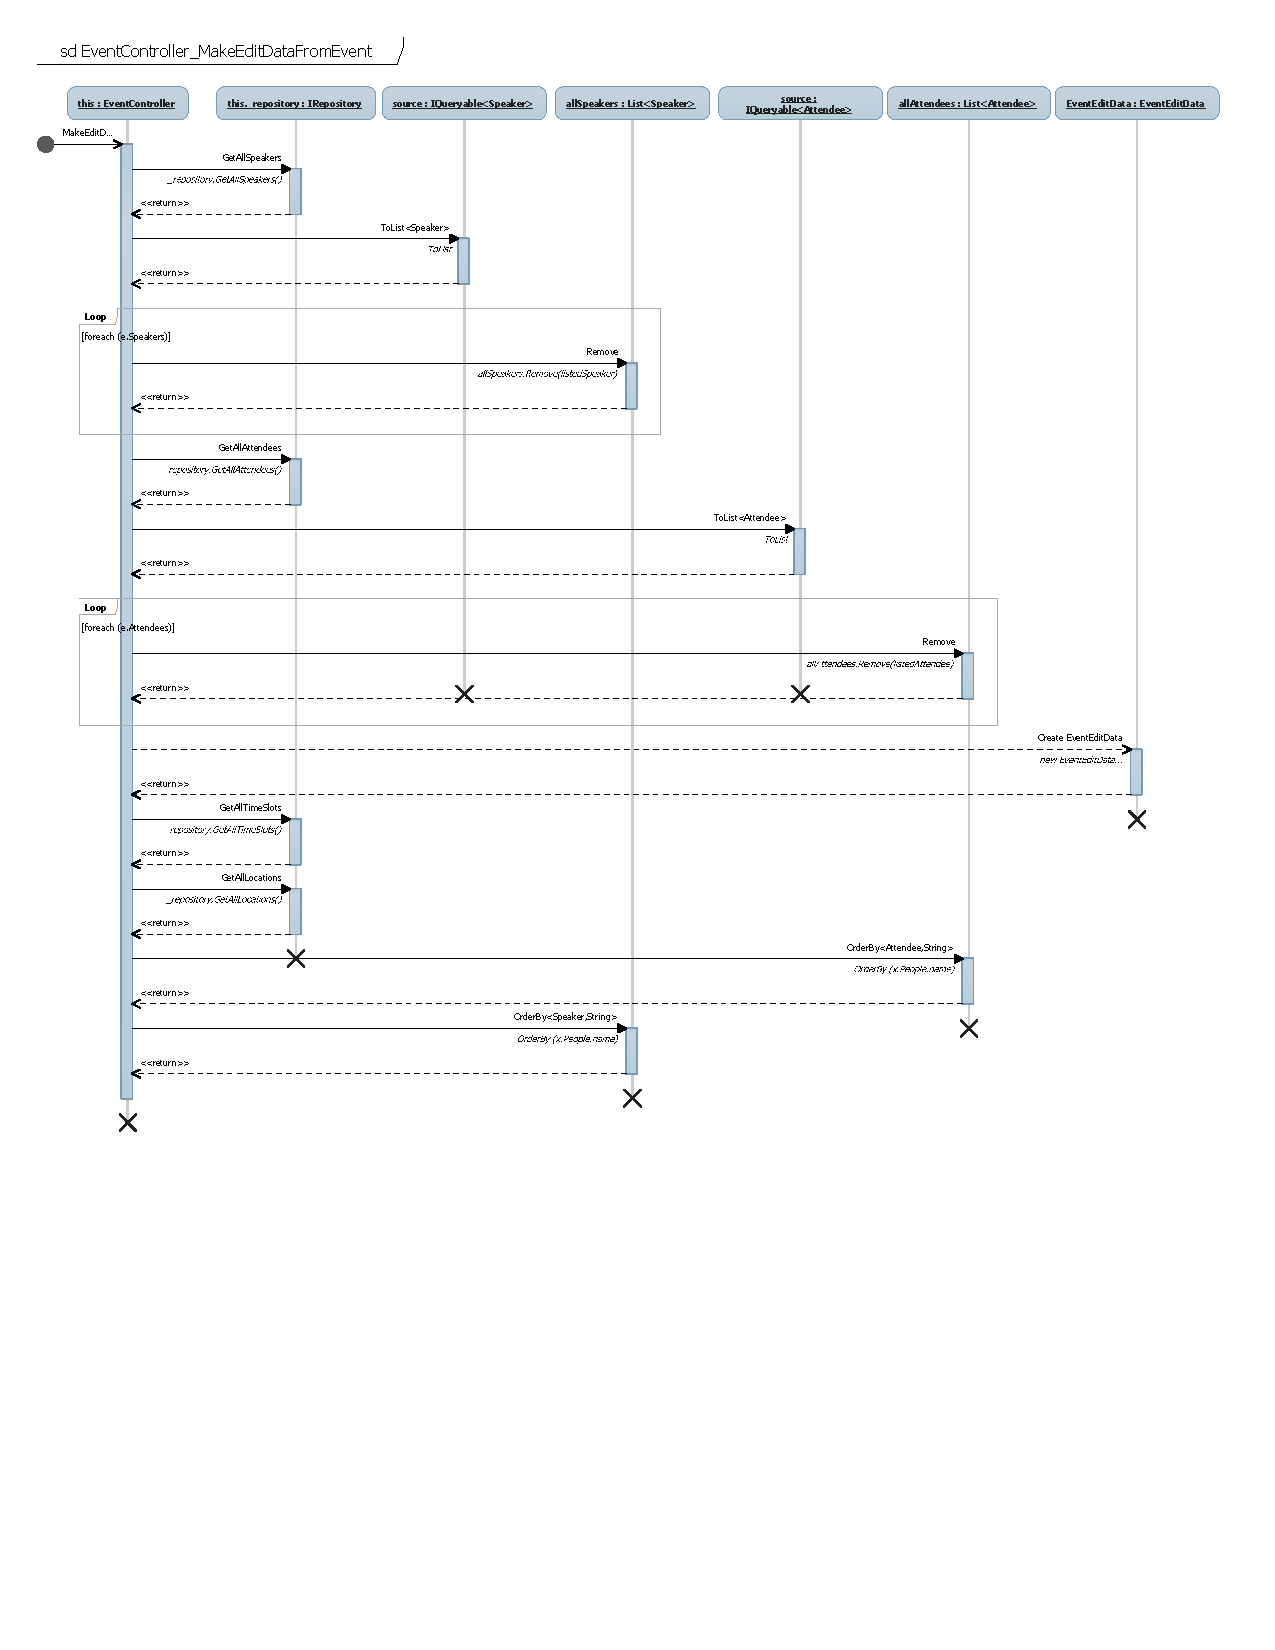
\includegraphics[scale=0.8]{ManageEvent_sequence}
\end{figure}
\newpage
\begin{figure}[H]
\centering
\caption{Register Attendee Sequence Diagram}
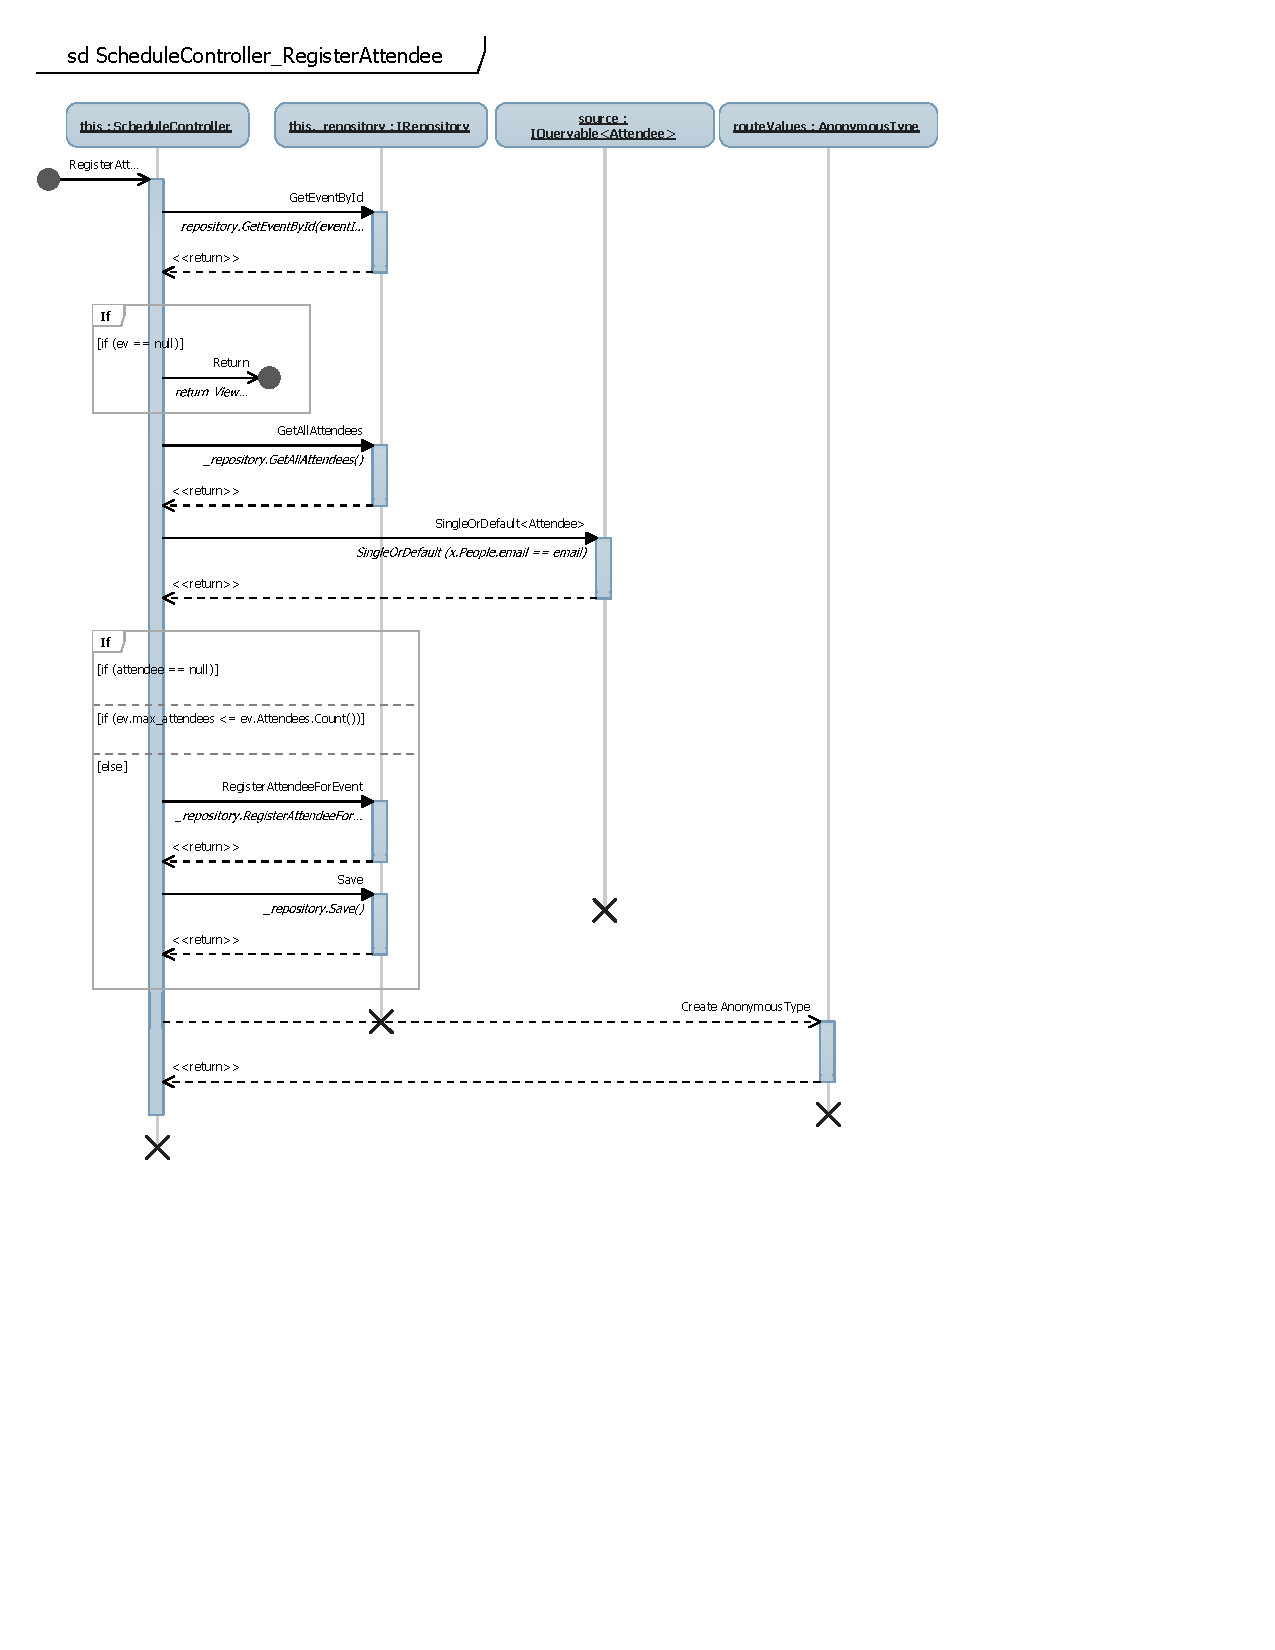
\includegraphics[scale=0.8]{RegisterAttendee_sequence}
\end{figure}
\newpage
\begin{figure}[H]
\centering
\caption{TShirtSize Create Sequence Diagram}
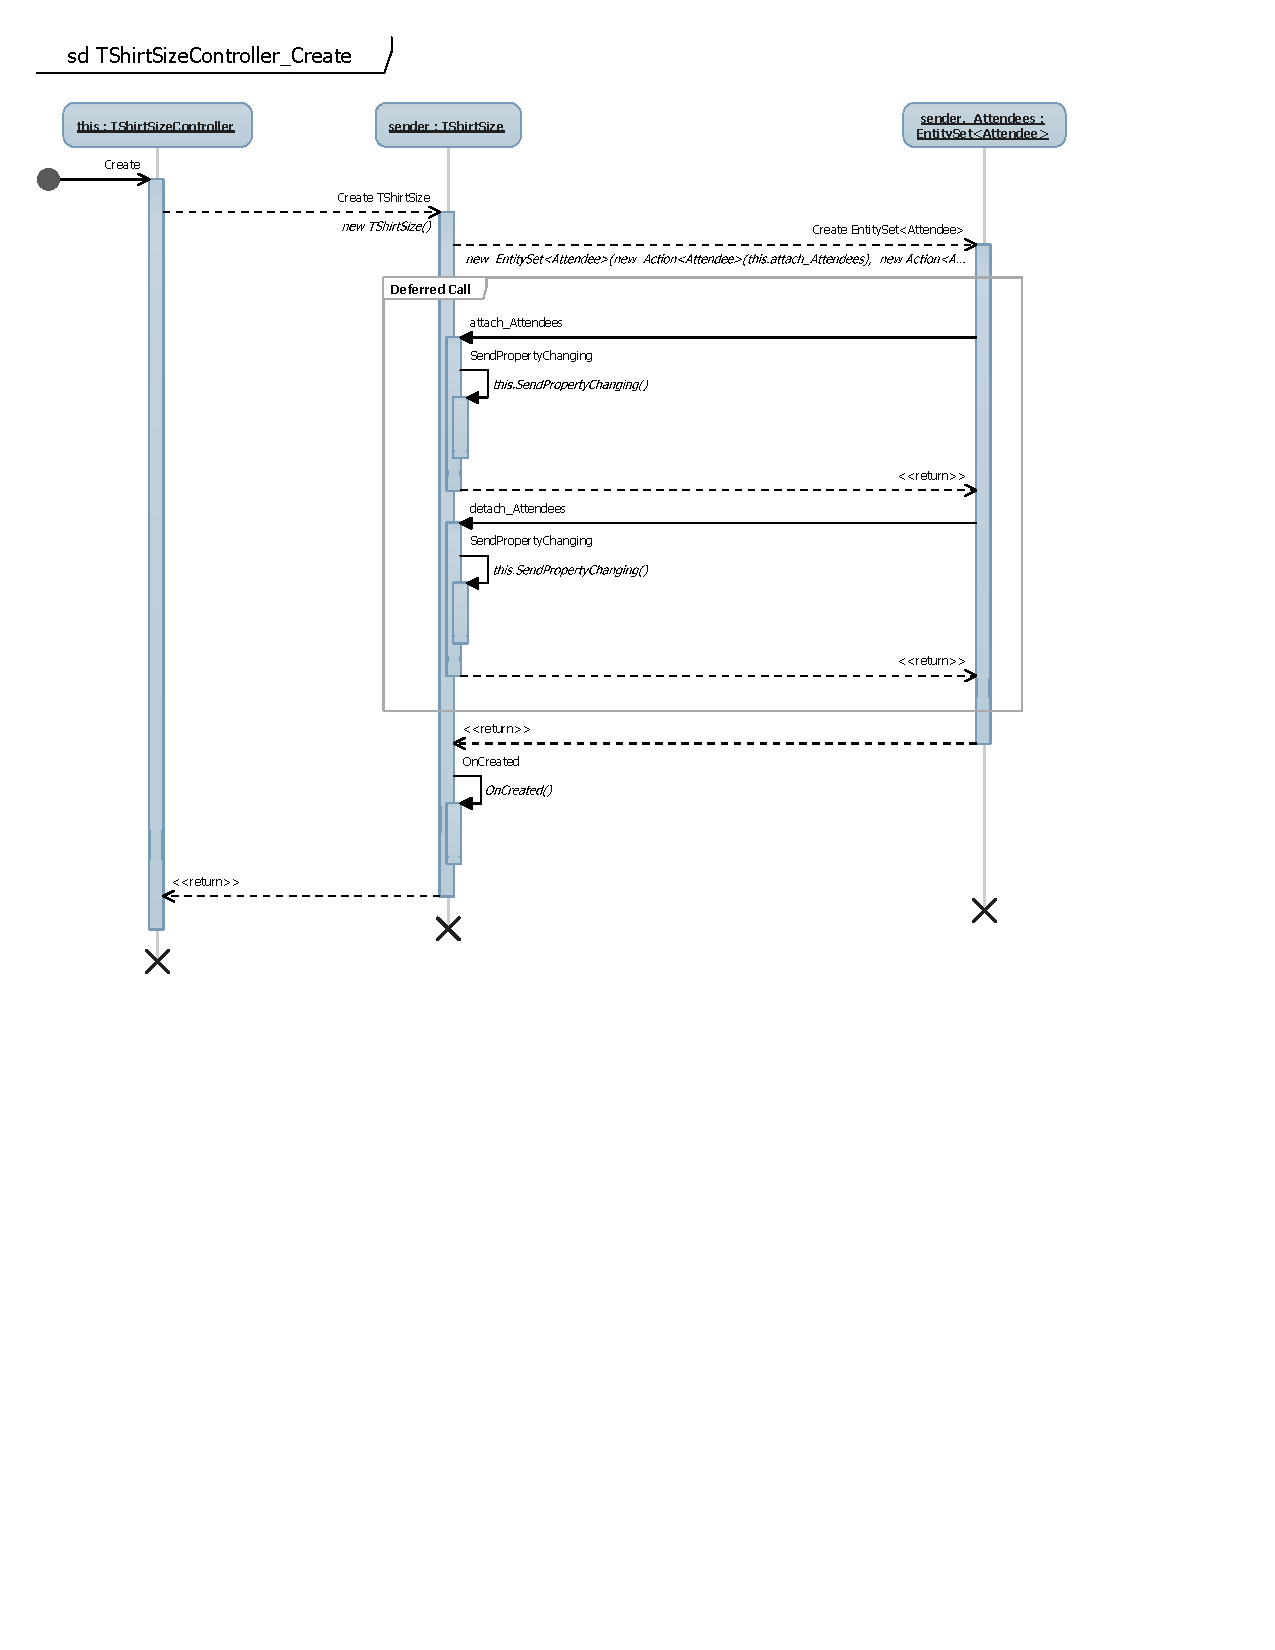
\includegraphics[scale=0.8]{TShirtSizeCreate_sequence}
\end{figure}
\newpage
\subsection{UML Class Diagram}
\begin{figure}[H]
\centering
\caption{UML Class Diagram of Conferenceware}
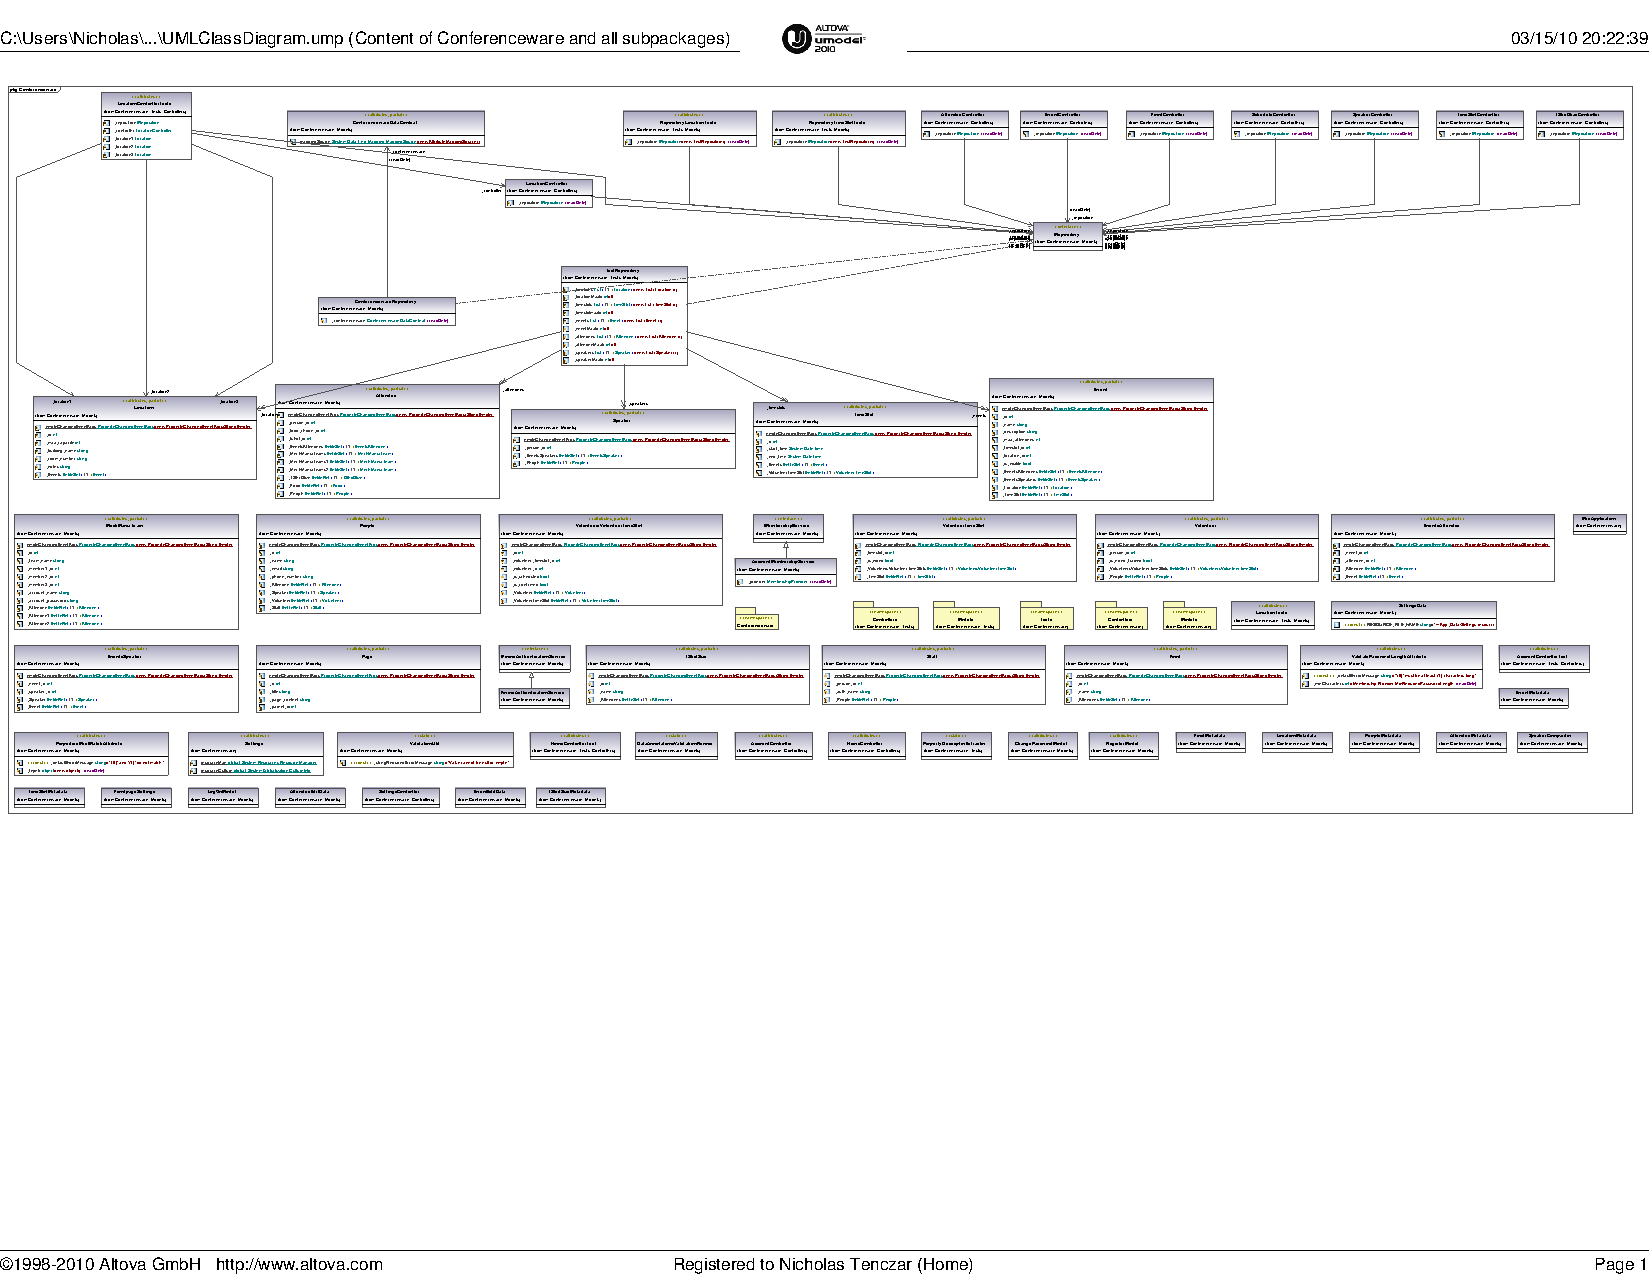
\includegraphics[width=\textwidth]{UMLClassDiagram}
\end{figure}

\newpage

\subsection{Design Explanation}
%% Jim's WA6

When we approach a large project, we must keep the entire design in mind all the time. Because Conferenceware is a project of considerable size and complexity, we need to keep conventions and separation consistent throughout the development process. Otherwise, we can not keep it 
in a manageable state. We strive to maintain cohesion when dealing with issues as course-grained as file management and as specific as module management or the content of the classes.  Our concern for consistent design extends to all aspects of the project.

We deal with literally hundreds of files for the main project alone, and supplemental changes (e.g., tests and documentation) add many more. Therefore, it is imperative to keep track of things. When writing Conferenceware, we use the language C\#, which can both hinder and facilitate our efforts.  C\# is very tolerant of different project structures. On the bright side, this means that we can choose to manage our files as we see fit most of the time, and the language will still understand and work flawlessly. But we can also make mistakes or poor decisions that the language will happily tolerate. Our choice in framework for the project, ASP.NET MVC, does impose two constraints for files, but the rest is a system respectd by everyone working on the project. The framework automatically creates folders that it suggests have certain uses. For instance, it provides a folder \texttt{App\_Data}, which is supposed to be used for private data (data which is not to be made
public to users on the internet).  The other folder that ASP.NET MVC provides is called Content, and it is where static files such as images or movies should be placed so they are accessible to users. There are also folders for Models (not actually enforced), Views, and Controllers. Controllers must all appear in the Controllers folder in the correct module (which is discussed below) and end with \texttt{Controller} in the file name. To make the \texttt{Dog} controller, the file would have to be named \texttt{DogController}. Views are also enforced to be in the Views folder. Inside of that folder, there are folders for each controller. Per the example e, there would also be a folder named \texttt{Dog} inside of Views. This folder is where views specific to that controller must live. The only alternative is to use the special folder called Shared where files are made available to every controller.

This framework is a good beginning for files, but it is not extensive enough to keep everything in order, even if we adhere to every suggestion. We must implement additional rules to keep the project organized. Let us examine a simple example concerning views. Each controller has its own directory for its own views. We do come across certain conditions, however, when one view is needed by multiple controllers: for example, an error page for when a requested item is not found. If two controllers deal with this item (which is not completely rare when the controllers are closely related, as they are with \texttt{Companies} and \texttt{Invoices}), we should choose to reuse the same file rather than duplicating it. o we keep a single version in \texttt{Shared}. We are then generally more able to limit the size of the \texttt{Shared} folder. On the other hand, we also uphold the rule that each class in the project is written in its own file even if it is small and only used in a single place. This increases the amount of files by a large amount. We insist on it because it makes finding classes much easier. We treat static files in a way that is similar to views, though Conferenceware can generally handle these files pragmatically on its own. Each event may well have content specific to the event (such as a recording of the event or any hand outs that were provided). We keep a folder in \texttt{Content} for each event when it is added by the system. There are also static shared files. These can be things such as the site's style sheet or common JavaScript files. We keep these files in the root of \texttt{Content} which also shortens the file path (and can actually speed up web page load times). We do give users the option to organize content differently so long as it still is in the \texttt{Content} folder. We anticipate that there might be common hand outs between events: one speaker might give both a general talk and a very technical workshop. We might also have several files for a given event, including example files. n our administrator t want to categorize the files into folders. We can accomplish all of this by adjusting file locations manually on the file system outside of Conferenceware and then allowing the administrator to simply provide static links to the files. Our set-up provides the user with a great deal of flexibility while still maintaining logic and order within the files. We also uphold one final rule, which is that classes are placed in the folder of their module (so any class in the \texttt{Conferenceware.Utils} module will have its file located in the \texttt{Utils} directory inside of the \texttt{Conferenceware} directory). We want to have enough verbosity to find the files but still be able to keep track of them all quite easily, and this system fulfills that goal.

Moving to a more fine-grained idea, we have developed a design for creating and maintaining modules which ensures a complete and effective application. There are many parallels between our approach to files as described above and our module management. A module is a collection of classes that are grouped together. We must evaluate when to keep classes together and when to separate them.  We consider several factors when evaluating this problem; it is not just a matter of minimizing typing. We take the idea of reusability to heart. Though we might never reuse certain parts of the project on their own, others might be useful - in particular, the models. These classes represent the data that is handled in the Conferenceware universe. They could benefit another developer who wants to create a separate conference management system or even just one who wants to integrate with Conferenceware. We want to be certain that all of the files used in managing data are in this module. We also want to include classes containing metadata about each of these classes. The metadata provides a more complete picture about the data and how it should and should not be used. If we omit it, there is ambiguity and an otherwise incomplete system. Some classes that are created for Conferenceware do not exactly fit with the rest. Sometimes this is very stark such as with the \texttt{Mailer} class. This class exists for the sole purpose of sending email based on certain settings in an environment with \texttt{SettingsData}. It doesn't actually display anything, control anything (as a controller does), or manage data. It functions as a utility, so it has been placed in \texttt{Conferenceware.Utils} with things that have a similar purpose. These classes generally exist to help with a single action and nothing else. We have come across some subtle differences when trying to display a picture to the screen. Normally we use controllers to render a view or, when they are done processing, to redirect to a different action. When we want to display a picture, it is like a simple view in some ways, but we must also convey some additional data. Because of this special case, we needto create a special result. It essentially functions in addition to the controllers (and is required by the controllers for them to function). These classes do not function on their own at all, and as such actually sit in the Controllers module. Again, we weigh how reusable these classes would be by themselves. By posing this simple question, we are able to keep modules reasonable, and the project remains much more manageable as it grows.

At the lowest, most specific level that we can manage with C\#, we must plan the design of individual classes. We decide which classes should be created and then what should be placed into them. When working through the latter problem, we remember that what is placed into each class is very directly related to the data it manages. In fact, we are using a library called LINQ (Language INtegrated Query) which gives a direct mapping between classes in Conferenceware and tables in the database. This allows us to manipulate our data very directly. Often, we may want to add some additional features beyond just data accessors to a class.  Sometimes we accomplish the objective through data processing. This can be used for converting internal data into something more functional, such as getting just the filename from a full file path. Alternatively, it might be able to convert unprocessed data like raw input from the user into something that is usable by the system internally.  In theory, we would naturally want to pair these methods with the class which stores the processed data.  t we find that they are sometimes even more useful as helper classes, so that multiple classes can use them independently but as a collection of similar data processing methods. Conference creates extra classes rather often simply because C\# is a strongly typed language. As developers, we can profit by exploiting this; we are able to find bugs earlier and create more reusable data.  For instance, when creating an event, we need to keep track of all the data in the event as well as a full list of locations and all the times that are available for holding the event. Thus we have created a class called EventEditData that holds these three aspects. It allows all of the views to generate certain aspects for the developer and validate data much more simply. When processing data or handling other aspects of event management, we might need the same data again. We can now just invoke the same class an additional time instead of being inconsistent. This does create additional classes to manage, but it keeps the overall development experience very verbose and therefore very predictable. Such predictability also massively increases maintainability. All of these aspects culminate to allow us to create a better project.

As a project grows, its design is tested. Conferenceware has shown that a well defined and very verbose design can stand up to a lot of growth of a code base. Conferenceware is therefore free to grow to become a full featured application which can be used and maintained for the future. Instead of being a source of frustration and constraints, a good design can bring tremendous benefits to a project.

\newpage
\section{Future Plans}
\subsection{Fate of the Code}
Conferenceware is planned to be used for many years to host the ACM Reflections $|$ Projections Conference. To facilitate the usage of this software, the whole project will be uploaded to GitHub, and have a UofI/NCSA License attached to it. Future generations of ACM members will hopefully maintain the project through updates of IIS, SQL Server, and ASP .NET MVC. There will be some future development of the project after class by the original Conferenceware team, but this will be very minor. The ACM Conference group is expected to be the future developers of the project after the middle of next semester.
\subsection{Future Features}
\subsubsection{Be able to email Volunteers their Schedule}
Volunteers are scheduled into specific time slots. It would be very useful to be
able to mass-send all of the volunteers their schedules once they have been
decided upon rather than needing to format them manually.
\subsubsection{Generate PDF Invoices}
Currently invoices are only generated as part of a web page (HTML). It would be
easier to email and is also preferred for many companies. Equivalent but nice
looking invoices would be good.
\subsubsection{Be able to email invoices}
Invoices have to be manually sent currently. Being able to send them easier
would be nice as well as keeping track of when they were last sent
\subsubsection{Create a way to keep track of email}
Though minor, keeping a full history of the emails sent would be good to do. For
historic reasons and just in case there is some confusion.
\subsubsection{(Auto) close registration}
Currently there is no way to close registration. When setting the flag to close
registration, it should be easy to give date and registration count to close
the registration without further input.
\subsubsection{Attendees can be checked in}
When an attendee arrives, we want to make sure to record that t-shirt and
program has been given to the person. We also need to be able to undo these
actions.
\subsubsection{Add a way to optionally enforce link locations}
Because of nginx, links might be different than what we expect. We should allow
links to be anything if the administrator desires.
%%TODO:fix these
\subsection{Personal Reflections}
\subsubsection{Eric Dyoniziak}
Overall, I found this project a great learning experience.  I have done previous web
development work but never using so many frameworks and tools.  I was amazed at how much
convience these tools provide, inparticular LINQ and the ASP.NET MVC Framework. Despite 
having learning curves they made development rather straightforward. Another valuable
experience was working with such a large group.  It put a realistic feel to the project
considering most software is developed in large groups and it had its own challenges to
learn from. This project also provided good exposure to software engineering techniques
used for starting up projects including requirements, design, architecture and teamwork.
All in all I'm very satisfied with my experience and I think as a group we succeeded in
creating a wonderful product. 
\subsubsection{Dan Freedman}
This project was quite an enlightening experience into the world of software engineering.
For the first time, I've had to work on a software project with more than just 2 or 3 people,
which was really a new experience. It made me realize how important constant communication
is to such a large project, and just how important a ticket management system is. I don't think
we would have gotten very far without Redmine, with its ability to do ticket modification from
Git commit messages. I've also learned from this project just how much better git is than svn,
and the ability to make quick and easy branches to test new functionality without breaking the master.
Git enabled us as a team to work more effectively, with powerful merge tools and greater per file controls.
I do not think that this project would have been as successful as it was if we were using svn.
\subsubsection{Stoyan Gaydarov}
I have been apart of Conference since I transfered into U of I and both years
we had to touch the database manually to get some of the information out of it.
This was not acceptable and when jim suggested this as our 428 project I was
really excited. I think that having our online ticket management helped with
keeping track of all the things that had to be done, and how far along things were.
I will be around next year when we are using this for the actual conference. I know
all the documentation we have done and all the tests we created are going to be
very helpful when we are trying to work with the system. Overall I am glad there
won't be any manual sql queries to remember to check how many volunteers we have.
\subsubsection{Simo Leone}
I've learned a lot while working on ConferenceWare. Before this project, and
being sort of a FOSS junkie myself, I had little or no experience with
C\#, ASP.NET, MSSQL, or even Visual Studio. Throughout the course of the project,
I learned all about partial classes in C\#, the garbled mess which is ASP syntax,
and the terrifying world of MSI installers. These technologies are in many cases
direct analogues to others which I was quite familiar with, which gave me a
whole new perspective on the usual web software stack. I'm glad to have had this
experience, since I feel that it makes me a more well-rounded and versatile
programmer, no matter what technology I may be working with in the future. In
addition, the project gave me an opportunity to work through a full project
with a team using development processes which I haven't had a lot of exposure
to before. While I do have some real-world experience, I can't say I've ever
had an excuse to make UML diagrams and proper use-case diagrams before. I
think this experience will be a great help in the future if I'm ever designing
something from scratch, since I'll have some exposure to software development
processes useful during the early stages of the software lifecycle. All in all,
I've greatly enjoyed working on ConferenceWare, and think the experience will
be quite beneficial in the future.
\subsubsection{Dave Paola}
\textit{Add personal reflections here}
\subsubsection{Brian Sawicki}
Working on this project was very different than my previous software engineering experience.  While in my internships the previous two summers I have worked on teams of comparable size, this was my first time developing a serious application in an entirely windows environment, meaning there were a lot of technologies being used that I was unfamiliar with.  I came in with only minor web development experience, as much of my prior work is in distributed systems, and I'm several years removed from the experience I do have.  This was also only the second time I had ever developed anything using C\# as the primary language.  All this combined made working on this project a real learning experience for me, full of new and sometimes frustrating problems to solve.  Despite my internship experience had never had to do a lot of the things we needed to do for this project.  For instance, while I have written plenty of unit tests before, I had never been forced to write tests for anything using the MVC pattern before.  Thankfully many of the members of the team were quite knowledgeable and able to give me a hand with any technical problems I ran into.  In the end I feel it has been a very beneficial project to work on, and I have enjoyed watching as our final product took shape over time. In the end I don't feel like I will probably be doing a lot of windows based web development in the future, however having used the XP process while working on the project (in particular the documentation work we did and the use of the redmine reporting system for bugs/users stories/etc) will almost certainly be invaluable after I graduate and join the workforce.
\subsubsection{Nick Tenczar}
\textit{Add personal reflections here}
\subsubsection{Jim Wordelman}
For me, this was not the first attempt at this project, but it was the first
successful creation. I had been in charge of maintaining the Conference web site
for the past two years directly and worked on it before that as well. This made
me extremely aware of how important and useful this project could be. Beyond
that, working on this amount of code with a team was a good experience. I became
very consistant about committing changes and keeping tickets up to date. This, I
forsee, will be invaluable in the future. Keeping a good level of communication
and all of the work was a great experience. I am very pleased with the outcome.
\newpage
\section{Appendix}
\subsection{Installation}
There is an installer for the project as a whole. There are some expectations
about the state of the system before it is installed though.
\begin{enumerate}
\item Microsoft SQL Server 2008 SP1 is installed on the same machine as the web
server
\item There is a Conferenceware database (named Conferenceware) in existance and
the installing user has full control over it
\item Internet Information Services (IIS) is installed an running with the
following roles: Static files, ASP.NET, and IIS 6 Metabase Compatibility
\end{enumerate}

The installer can then just be run. A database will be created and an
administrator will be added with the credentials provided during the install.
After the install, the user that is running ASP.NET on the local system will
need to be given access to the database. This reminder is given at the end of
installation.
\subsection{How to run}
After running the installer and fixing the database permissions, the system is
running any time the web server is running with the website into which
Conferenceware was installed. All one has to do is navigate to the web site (for
instance http://localhost/Conferenceware). From here, the administrator can log
in with the credentials specified in the installer and begin to configure the
conference (by going through settings and events and so on).
\end{document}
